\section{Hardware}
\subsection{Technische Daten der Lichtschranke}
\null\marg{Lichtschranke}
\begin{tabular}{ll}
    Hersteller & Panasonic\\
    Typ & Einweglichtschranke\\
    Modellnummer &  EX-21A-PN \\
    Schalttyp & Hell-EIN\\
    Reichweite & 1m\\
    Wiederholpräzision & max. 0.05mm\\
    Ansprechzeit & max. 0.5 ms\\
    Spannung & max 30V\\
    Stromaufnahme & max. 10mA
\end{tabular}
\\
Die kompletten Technischen Daten findet man in Anhang \ref{app:ex20}.

\subsection{Arduino}
Als \marg{Arduino Uno} Embedded System wird ein Arduino Uno verwendet. Er wird wie in \ref{fig:ArdAns} gezeigt angeschlossen.  Die Berechnung zum Spannungsteiler findet sich im Anhang \ref{app:berechnung}.

\begin{figure}[ht]
    \centering
%    \missingfigure{Bild einfügen}
    	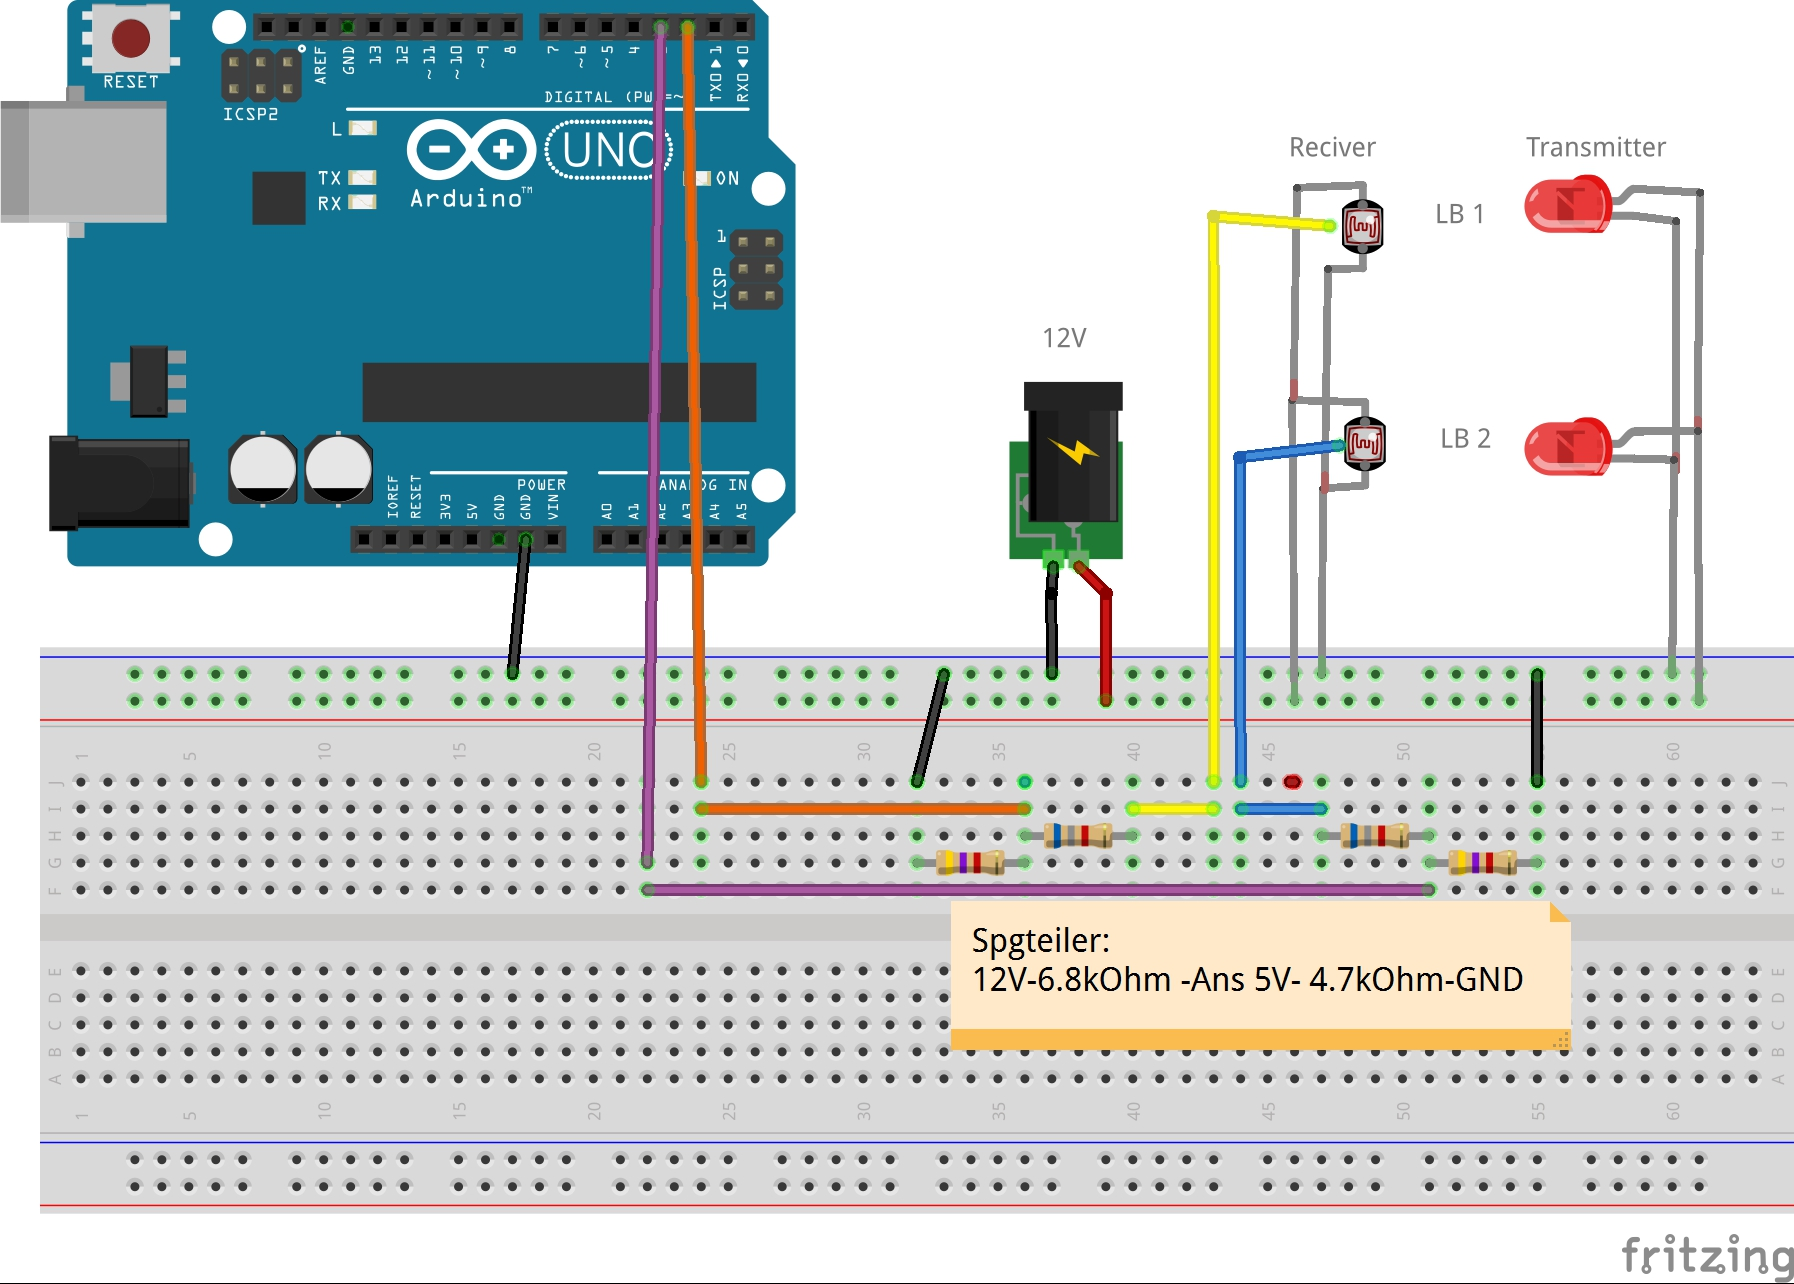
\includegraphics[width=\textwidth]{images/fritzing.jpg}
    \caption{Anschluss des Arduino Uno}
    \label{fig:ArdAns}
\end{figure}
Anschluss\enlargethispage{\baselineskip}\marg{Anschluss}:\newline
\begin{tabular}{ll}
    \textbf{Pin} & \textbf{Bezeichnung}\\
    2 & Lichtschranke 1 (LB1)\\
    3 & Lichtschranke 1 (LB1)\\
\end{tabular}